\documentclass[lang=cn,12pt, scheme=chinese]{elegantbook}


\usepackage{amsmath}
\usepackage{slashed}
\usepackage{mathtools}
\usepackage{cancel}
\usepackage{wrapfig}
\usepackage{tikz}
\usetikzlibrary{positioning, shapes.geometric, arrows.meta}
\usepackage{ulem}
%\usepackage{CJKulem}
\usepackage{xeCJK}
\usepackage{CJKfntef}


\title{课程学习笔记}
% \subtitle{Classic Elegant\LaTeX{} Template}

\author{S.Y. Chen}
\bioinfo{单位}{Southwest University}
\bioinfo{时间}{\today}
% \institute{Southwest University}
% \date{\today}
% \version{3.11}
% \bioinfo{Bio}{Information}

\extrainfo{Victory won\rq t come to us unless we go to it. }

\logo{logo-blue.png}
\cover{cover.jpg}

\begin{document}

\maketitle

\frontmatter
\tableofcontents

\mainmatter

%%%%%%%%%%%%%%%%%%%%%%%%%%%%%%%%%%%%%%%%%%%%%%%%
\part{数学基础}
%%%%%%%%%%%%%%%%%%%%%%%%%%%%%%%%%%%%%%%%%%%%%%%%%%%%%%%%%%%%%%%%%%%%%
\chapter{坐标系}



\part{群论}
\chapter{群与群表示理论}

%%%%%%%%%%%%%%%%%%%%%%%%%%%%%%%%%%%%%%%%%%%%%%%%%%%%%%%%%%%%%%%%%
\section{群的基本概念与性质}
\begin{definition}{群的定义:}
	设$G$是一些元素的集合,$G = {\cdots, g, \cdots,} = {g}$。在$G$中定义了乘法运算。$G$构成一个群所满足的条件为:
	\begin{enumerate}
		\item 封闭性。即对任意元素$f, g \in G$,若$ h = fg$也有$h \in G$。
		\item 结合律。对任意$f, g, h \in G$,都有
			\begin{equation*}
				(fg)h = f(gh)
			\end{equation*} 
		\item 有唯一单位元素。即有$e \in G$,对任意$f \in G$,都有
			\begin{equation*}
			    ef = fe = f
			\end{equation*} 
		\item 有逆元素。即对任意的$f \in G$,都有唯一的$ f^{-1} \in G$,满足
			\begin{equation*}
				f^{-1} f = f f^{-1} = e
			\end{equation*} 
	\end{enumerate}
	其中,$e$为群$G$的单位元素,$f^{-1}$为$f$的逆元素。
\end{definition}
构成群的可以是一些操作,比如一些集合的置换和三角形的空间变换等,以下举例说明:
\begin{example}
	$n$阶置换群$S_n$,又称$n$阶对称群。将$n$个元素
\end{example}
\begin{example}	\label{exp:D3_group}
	平面正三角形对称群$D_3$,又称为6阶二面体群。考虑中心在原点,底边与$x$轴平行的$xOy$平面上的正三角形$\bigtriangleup ABC$,见图\ref{fig:D3_group_fig}。保证三角形空间位置不变的操作有:
	\begin{equation*}
		\begin{aligned}
			e&\text{:保持三角形不动;}			\quad	&d\text{:绕$z$轴转动$2\pi/3$;}\\
			f&\text{:绕$z$轴转动$4\pi/3$;}	\quad	&a\text{:绕轴$1$转动$\pi$角;}	 \\
			b&\text{:绕轴$2$转动$\pi$角;}		\quad	&c\text{:绕轴$3$转动$\pi$角;}
		\end{aligned}
	\end{equation*}
	现在我们定义以上操作的乘积,如$ab$为先进行$a$操作再进行$b$操作。
	\begin{figure}[htbp]
		\centering
		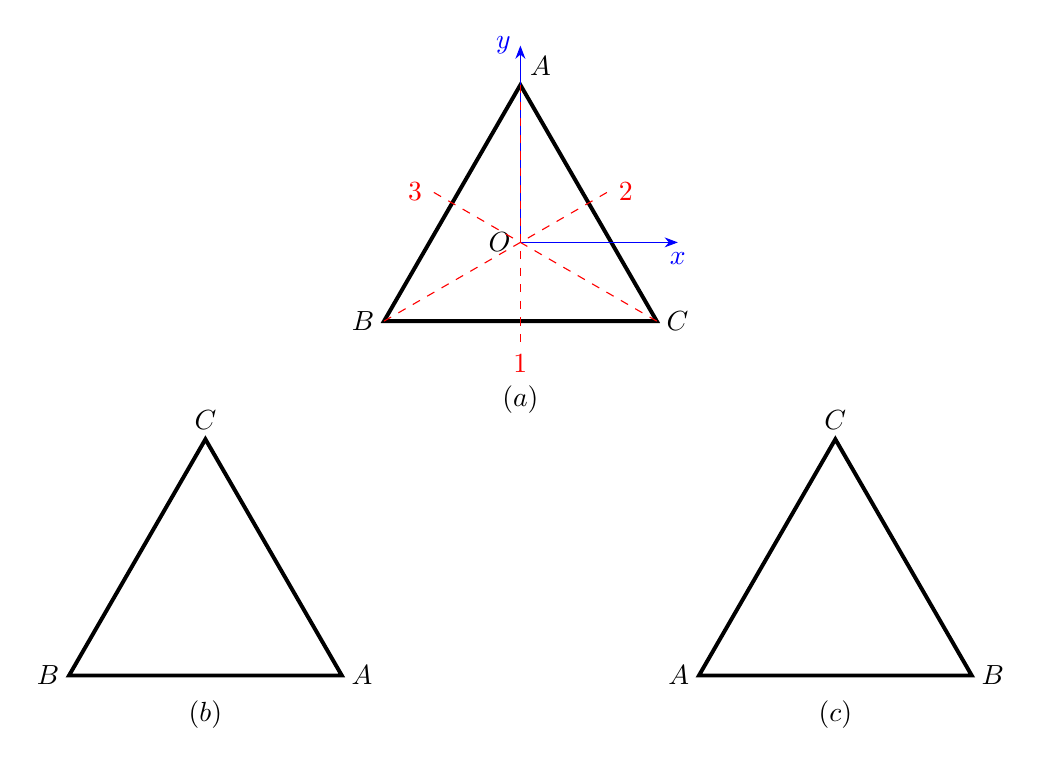
\begin{tikzpicture}
			\draw	[line width=.05cm]	(-1.732, -1) -- (1.732, -1) -- (0, 2) -- cycle;
			\node	(A)	at	(0, 2)			[above right]	{$A$};
			\node	(B)	at	(-1.732, -1)	[left]			{$B$};
			\node	(C)	at	(1.732, -1)		[right]			{$C$};
			\node	(O)	at	(0, 0)			[left]			{$O$};
			\draw	[-Stealth, blue]	(0, 0)		 --	(2, 0)		node[at end, below]{$x$};
			\draw	[-Stealth, blue]	(0, 0)		 --	(0, 2.5)	node[at end, left]{$y$};
			\draw	[red, dashed](0, 2) -- +(0, -3.3)	node[at end, below]{$1$};
			\draw	[red, dashed](-1.732, -1) -- +(30:3.3cm)	node[at end, right]{$2$};
			\draw	[red, dashed](1.732, -1) -- +(150:3.3cm)	node[at end, left]{$3$};
			\node	(a)	at	(0, -2)						{$(a)$};

			\draw	[line width=.05cm]	(-5.732, -5.5) -- (-2.268, -5.5) -- (-4, -2.5) -- cycle;
			\node	(A1)	at	(-2.268, -5.5)	[right]	{$A$};
			\node	(B1)	at	(-5.732, -5.5)	[left]	{$B$};
			\node	(C1)	at	(-4, -2.5)		[above]	{$C$};
			\node	(b)		at	(-4, -6)				{$(b)$};
			\draw	[line width=.05cm]	(2.268, -5.5) -- (5.732, -5.5) -- (4, -2.5) -- cycle;
			\node	(A2)	at	(2.268, -5.5)	[left]	{$A$};
			\node	(B2)	at	(5.732, -5.5)	[right]	{$B$};
			\node	(C2)	at	(4, -2.5)		[above]	{$C$};
			\node	(c)		at	(4, -6)				{$(c)$};
		\end{tikzpicture}
		\caption{正三角形转动操作}
		\label{fig:D3_group_fig}
	\end{figure}
	我们发现,对图中的三角形进行上述任意的六种操作以及相应的乘法操作,此\uline{三角形在空间上保持不变},如图\ref{fig:D3_group_fig}(b),它可以认为是直接对(a)进行$b$操作,也可认为是先进行$c$操作在进行$d$操作,这样,我们就可以得到这样的关系$dc=b$。在这些乘法作用下,上述这些操作构成群,我们称为\textcolor{red}{$D_3$群},其乘法表如下:
	\begin{table}[!ht]
		\centering
		\caption{$D_3$群乘法表}
		\setlength{\tabcolsep}{10mm}{
		\begin{tabular}{|c|cccccc|}\hline
			~	&	e	&	d	&	f	&	a	&	b	&	c	\\	\hline
			e	&	e	&	d	&	f	&	a	&	b	&	c	\\	
			d	&	d	&	f	&	e	&	c	&	a	&	b	\\	
			f	&	f	&	e	&	d	&	b	&	c	&	a	\\	
			a	&	a	&	b	&	c	&	e	&	d	&	f	\\	
			b	&	b	&	c	&	a	&	f	&	e	&	d	\\	
			c	&	c	&	a	&	b	&	d	&	f	&	e	\\	\hline
		\end{tabular} 
		}
	\end{table}
\end{example}


\section{群表示}
\subsection{群表示基础}
构成群的是一些操作,既然是一些操作,那么必然有其所对应的操作对象,其操作对象是位于某一空间下的,比如前面的例\ref{exp:D3_group},群元是一些操作,而这些操作所对应的对象则是位于三维空间中的正三角形;我们将此三角形在三维空间中表示出来(只表示其顶点坐标),那么它将以列矢的形式表现出来,而对应的群操作的表现形式则为矩阵,这些矩阵同样构成群。因此,我们可以说,\CJKunderdot{所谓的群表示就是某一群$G$到线性空间$V$上的某一线性变换群$L(V,C)$的同态映射,也就是说表示是一种同态映射关系,它存在于一个抽象群和线性空间的线性变换群之间。}

群中的群元是对某一个对象进行某种操作,而群表示则相当于我们要在某一个具体的空间下用数学的语言来描述这个群元所对应的操作。在理解这个操作之前需要了解线性空间和线性变换的概念。
\begin{definition}{线性空间(向量空间)}
	线性空间是定义在数域$\mathbb{K}$(比如实数域$\mathbb{R}$或复数域$\mathbb{C}$)上的向量集合$V = \{\bm{x}, \bm{y}, \bm{z}, \cdots\}$。在$V$中可以定义加法和数乘两种运算。设矢量$\bm{x}, \bm{y}, \bm{z} \in V$,数$a , b , c \in \mathbb{K}$,向量加法和数乘都具有封闭性,满足\newline
	向量加法:
	\begin{enumerate}
		\item $\bm{x} + \bm{y} = \bm{y} + \bm{x}$
		\item $\bm{x} + ( \bm{y} + \bm{z} ) = (\bm{x} + \bm{y}) + \bm{z}$
		\item 有唯一$\bm{0}$元素,$\bm{x} + \bm{0} = \bm{x}$
		\item 对$\forall \bm{x}$,有唯一的$-\bm{x}$,使得$\bm{x} + (-\bm{x}) = \bm{0}$
	\end{enumerate}
	向量与数的乘法:
	\begin{enumerate}
		\item $1 \cdot \bm{x} = \bm{x}$
		\item $(ab)\bm{x} = a(b\bm{x})$
		\item $a(\bm{x} + \bm{y}) = a\bm{x} + a\bm{y}$
		\item $(a + b) \bm{x} = a\bm{x} + b\bm{x}$
	\end{enumerate}
	现在把向量的加法看成群的乘法,则线性空间$V$构成一个可交换的加法群。
\end{definition} 
线性空间最简单的一个例子就是三维空间,若三维空间按笛卡尔坐标系展开,则上面的向量都可用$(x, y, z)$表示,而且具有封闭性,也就是这些向量相加或数乘都无法超过这个空间。
\begin{definition}{线性无关向量}
	线性空间$V$中,若任意$n$个向量$\bm{X}_1, \bm{X}_2, \cdots, \bm{X}_n$的线性组合$a_1\bm{X}_1 + a_2\bm{X}_2 + \cdots + a_n\bm{X}_n = 0$,其中$a_1, a_2, \cdots, a_n \in \mathbb{K}$,当且仅当$a_1 = a_2 = \cdots = a_n = 0$时成立,这时,称$\bm{X}_1, \bm{X}_2, \cdots, \bm{X}_n$这些向量线性无关。否则,称他们线性相关。
\end{definition} 

\begin{definition}
	线性变换$A$是将线性空间$V$映入$V$的映射,这个映射对$\forall \bm{x}, \bm{y} \in V$和$\forall a, \in \mathbb{K}$,满足$A(a\bm{x} + b\bm{y} = aA\bm{x} + bA\bm{y}$,也就是说这个变换作用到向量的线性组合上,等于这个变换作用到向量上的线性组合。
\end{definition}
所谓映射其实就是一种操作,它把某个区域的东西变成另一个区域的某样东西,上面的定义中$A$是将$V$中的某个元素变成$V$中的另一样元素,这两个元素可能相同也可能不同。这里,$A$将表现为矩阵形式,而我们所需要做的就是找到$A$所对应的矩阵。当我们取定$V$中的基矢为$\bm{e}_1, \bm{e}_2, \cdots, \bm{e}_n$时,对$V$中的某一向量$x=\sum_{i=1}^{n}x_i\bm{e}_i$做相关的线性变换,表现为
\begin{equation}
	\begin{aligned}
		A\bm{x} =& \sum_{j=1}^{n} x_j A \bm{e}_j = \sum_{j=1}^{n}\sum_{i=1}^{n} x_j e_i a_{ij}	\\
				=& (\bm{e}_1, \bm{e}_2, \cdots, \bm{e}_n)
					\begin{pmatrix}
						a_{11}	&	a_{12}	&	\cdots	&	a_{1n}	\\
						a_{21}	&	a_{22}	&	\cdots	&	a_{2n}	\\
						\vdots	&	\vdots	&	\ddots	&	\vdots	\\
						a_{1n}	&	a_{2n}	&	\cdots	&	a_{nn}	\\
					\end{pmatrix}
					\begin{pmatrix}
						x_1	\\
						x_2	\\
						\vdots	\\
						x_n
					\end{pmatrix}	\label{eq:group_basis_change}
	\end{aligned}
\end{equation}
我们知道,一个线性空间可选取不同的基矢,不同基矢之间可通过矩阵变换联系起来,上式第三个等号的左边两项可构成向量空间$V$的另一组基,我们考虑为$\bm{e}^{\prime}_1, \bm{e}^{\prime}_2, \cdots, \bm{e}^{\prime}_n$,它们之间的关系如下:
\begin{equation}
	\bm{e}^{\prime}_{j} = (\bm{e}_1, \bm{e}_2, \cdots, \bm{e}_n) 
						\begin{pmatrix}
							a_{1j}	\\
							a_{2j}	\\
							\vdots	\\
							a_{nj}
						\end{pmatrix}
\end{equation} 
下面,我们取$V$中另一向量$\bm{y} = \sum_{i=1}^{n}y_i\bm{e}_i$,它是$\bm{x}$通过映射$A$得到的,满足$\bm{y} = A\bm{x}$。对于$\bm{y}$,写成矩阵形式为
\begin{equation}
	\bm{y} = (\bm{e}_1, \bm{e}_2, \cdots, \bm{e}_n)
				\begin{pmatrix}
					y_1	\\
					y_2	\\
					\vdots	\\
					y_n
				\end{pmatrix}	\label{eq:group_basis_eq_change}
\end{equation} 
由于$\bm{y}$与$A\bm{x}$表示的是同一向量,联合式\eqref{eq:group_basis_change}和\eqref{eq:group_basis_eq_change},我们有以下关系成立
\begin{equation}
	 (\bm{e}_1, \bm{e}_2, \cdots, \bm{e}_n)
		\begin{pmatrix}
			a_{11}	&	a_{12}	&	\cdots	&	a_{1n}	\\
			a_{21}	&	a_{22}	&	\cdots	&	a_{2n}	\\
			\vdots	&	\vdots	&	\ddots	&	\vdots	\\
			a_{1n}	&	a_{2n}	&	\cdots	&	a_{nn}	\\
		\end{pmatrix}
		\begin{pmatrix}
			x_1	\\
			x_2	\\
			\vdots	\\
			x_n
		\end{pmatrix}
		=
		(\bm{e}_1, \bm{e}_2, \cdots, \bm{e}_n)
		\begin{pmatrix}
			y_1	\\
			y_2	\\
			\vdots	\\
			y_n
		\end{pmatrix}
\end{equation} 
由式\eqref{eq:group_basis_eq_change},我们用新基矢$\bm{e}^{\prime}_1, \bm{e}^{\prime}_2, \cdots, \bm{e}^{\prime}_n$替换上式等号的右边两个矩阵,也就是有下式成立
\begin{equation}
	(\bm{e}^{\prime}_1, \bm{e}^{\prime}_2, \cdots, \bm{e}^{\prime}_n )
	=
	(\bm{e}_1, \bm{e}_2, \cdots, \bm{e}_n)
	\begin{pmatrix}
		a_{11}	&	a_{12}	&	\cdots	&	a_{1n}	\\
		a_{21}	&	a_{22}	&	\cdots	&	a_{2n}	\\
		\vdots	&	\vdots	&	\ddots	&	\vdots	\\
		a_{1n}	&	a_{2n}	&	\cdots	&	a_{nn}	\\
	\end{pmatrix}
\end{equation} 
以上我们可以看出,通过矩阵$A$,我们可以把新基矢与旧基矢联系起来,矩阵的第$j$列,是新基矢用旧基矢表示的展开系数。这样,当我们知道新基矢与旧基矢之间的关系时(也就是\CJKunderdot{新基矢用旧基矢展开的展开系数}),我们就可以把矩阵$A$写出来,也就是可以把抽象群元对应的表示写出来。我们来看一个例子
\begin{example}
	以$D_3$群群元$b$为例,来考虑它在三维线性空间中的表示。首先,轴$2$在此空间中可表示为某一直线方程:
	\begin{equation}
	    -\tan \frac{\pi}{6} x + y = 0
	\end{equation} 
	而群元$b$是让三角形发生关于此直线的镜像变换,而原来的基矢为$\bm{e}_{x}, \bm{e}_{y}, \bm{e}_z$,变换后的基矢为$\bm{e}^{\prime}_x, \bm{e}^{\prime}_y,\bm{e}^{\prime}_z$,它们之间的关系由下图表示
	\begin{figure}[htbp]
		\centering
		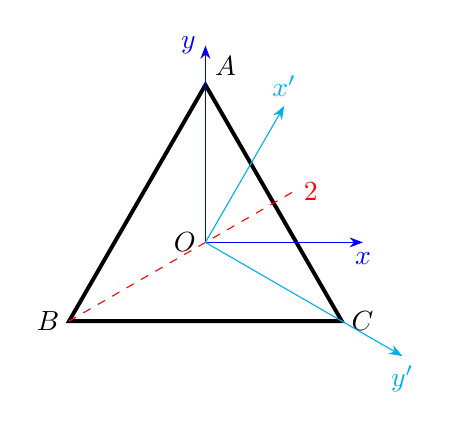
\begin{tikzpicture}
			\draw	[line width=.05cm]	(-1.732, -1) -- (1.732, -1) -- (0, 2) -- cycle;
			\node	(A)	at	(0, 2)			[above right]	{$A$};
			\node	(B)	at	(-1.732, -1)	[left]			{$B$};
			\node	(C)	at	(1.732, -1)		[right]			{$C$};
			\node	(O)	at	(0, 0)			[left]			{$O$};
			\draw	[-Stealth, blue]	(0, 0)		 --	(2, 0)		node[at end, below]{$x$};
			\draw	[-Stealth, blue]	(0, 0)		 --	(0, 2.5)	node[at end, left]{$y$};
			\draw	[red, dashed](-1.732, -1) -- +(30:3.3cm)	node[at end, right]{$2$};

			\draw	[-Stealth, cyan]	(0, 0)		 --	(1, 1.732)		node[at end, above]{$x^\prime$};
			\draw	[-Stealth, cyan]	(0, 0)		 --	(2.5, -1.4434)	node[at end, below]{$y^\prime$};
		\end{tikzpicture}
		\caption{$D_3$群群元$b$在三维空间中的操作}
	\end{figure}
	\newline
	写成数学表达式:
	\begin{equation}
	    \begin{aligned}
			\bm{e}_x^\prime =& \cos \frac{2\pi}{6} \bm{e}_x + \sin \frac{2\pi}{6} \bm{e}_y	\\
			\bm{e}_y^\prime =& \sin \frac{2\pi}{6} \bm{e}_x - \cos \frac{2\pi}{6} \bm{e}_y	\\
			\bm{e}_z^\prime =& \bm{e}_z
	    \end{aligned}
	\end{equation} 
	根据上式写成矩阵形式,则可得到$D_3$群元$b$在三维线性空间中的群表示
	\begin{equation}
	    A(b) =
		\begin{pmatrix}
			\cos \frac{2\pi}{6}	&	\sin \frac{2\pi}{6}		&	0	\\
			\sin \frac{2\pi}{6}	&	-\cos \frac{2\pi}{6}	&	0	\\
			0					&	0						&	1	
		\end{pmatrix}
	\end{equation} 
\end{example}

\begin{definition}
	设有群$G$,如存在一个从$G$到$n$维线性空间$V$上的线性变换群$L(V,C)$的同态映射$A$,则称$A$是群$G$的一个线性表示,$V$为表示空间,$n$是表示的维数。显然,由同态的定义,$\forall g_\alpha \in G$,有$A(g_\alpha) \in L(V, C)$,同时,对$\forall g_\alpha, g_\beta \in G$,有$A(g_\alpha g_\beta) = A(g_\alpha)A(g_\beta)$。$G$的单位元素对应的是$V$上的恒等变换,互逆元素对应的是互逆的变换。
\end{definition}
\CJKunderdot{对于线性空间$V$,如果选定一组特定的基矢,那么每个线性变换都可以有一个矩阵表示,而线性变换也会对应到一个矩阵群。这是,抽象群$G$与线性变换群的同台映射关系可以理解为抽象群$G$与矩阵群的同态映射关系。}我们考虑一个例子来理解这个概念,同样取例\ref{exp:D3_group},我们在三维笛卡尔坐标系中对其展开描述,$D_3$群群元对应到线性空间中的矩阵为
\begin{equation*}
	\begin{aligned}
		&e \xRightarrow[]{A}
		A(e) = 
		\begin{pmatrix}
			1	&	0	&	0	\\
			0	&	1	&	0	\\
			0	&	0	&	1
		\end{pmatrix}
		\\
		&d \xRightarrow[]{A}
		A(d) =
		\begin{pmatrix}
			\cos \frac{2\pi}{3}	&	\sin \frac{2\pi}{3}	&	0	\\
			-\sin	\frac{2\pi}{3}	&	\cos \frac{2\pi}{3}	&	0	\\
			0	&	0	&	1
		\end{pmatrix}
		\\
		&f \xRightarrow[]{A}
		A(d) =
		\begin{pmatrix}
			\cos  \frac{4\pi}{3}	&	\sin \frac{4\pi}{3}	&	0	\\
			-\sin \frac{4\pi}{3}	&	\cos \frac{4\pi}{3}	&	0	\\
			0						&	0					&	1
		\end{pmatrix}
		\\
		&a \xRightarrow[]{A}
		A(a) =
		\begin{pmatrix}
			-1	&	0	&	0	\\
			0	&	1	&	0	\\
			0	&	0	&	1
		\end{pmatrix}
		\\
		&b \xRightarrow[]{A}
		A(b) =
		\begin{pmatrix}
			\frac{1}{2}			&	\frac{\sqrt{3}}{2}	&	0	\\
			\frac{\sqrt{3}}{2}	&	-\frac{1}{2}		&	0	\\
			0					&	0					&	1
		\end{pmatrix}
		\\
		&c \xRightarrow[]{A}
		A(c) =
		\begin{pmatrix}
			\frac{1}{2}			&	-\frac{\sqrt{3}}{2}	&	0	\\
			-\frac{\sqrt{3}}{2}	&	-\frac{1}{2}		&	0	\\
			0					&	0					&	1
		\end{pmatrix}
	\end{aligned}
\end{equation*} 
其中,$A$是一种映射关系,它将$D_3$群中的群元在线性空间中表示为矩阵,而这些矩阵是属于线性变换群$L(V,C)$的。这样,我们可以把群表示关系(抽象群与矩阵变换群的关系)写成如下形式:
\begin{figure}[htbp]
	\centering
	\begin{tikzpicture}
		\draw	(-3, 0)ellipse [x radius=1.2cm, y radius=2cm];
		\draw	(3, 0)ellipse [x radius=1.2cm, y radius=2cm];
		\draw	[-Stealth]	(-2.8, 0.7)	--	(2.8, 0.7);
		\node	(g_alpha)	at	(-2.9, 0.7)	[left]	{$g_{\alpha}$};
		\node	(A_alpha)	at	(2.9, 0.7)	[right]	{$A(g_\alpha)$};
		\node	(G)	at	(-3, 2.5)	{$G$};
		\node	(L)	at	(3, 2.5)	{$L(V,C)$};
		\node	(A)	at	(0, 2.5)	{$A$};
	\end{tikzpicture}
	\caption{群表示}
\end{figure}
\newline
下面,我们举一些例子一边更好的理解清楚这个定义的概念
\begin{example}
	考虑三个二阶群:(1) $\{E, \sigma_k\}$(三维空间对$x-y$平面的反射),(2) $\{E, C_k(\pi)\}$(绕$z$轴转$\pi$角),(3) $\{E, I\}$(空间反演操作)。去表示空间为三维实空间,基矢为$\{\bm{i}, \bm{j}, \bm{k}\}$,写出它们的表示。首先,我们考虑群元$E$,由于它是恒等变换,也就是把$\{\bm{i}, \bm{j}, \bm{k}\}$变成$\{\bm{i}, \bm{j}, \bm{k}\}$,对应的新向量在旧基矢组下的展开系数分别为$(1, 0, 0), (0, 1, 0), (0, 0, 1)$,表示矩阵为三阶单位矩阵。
	\newline
	对于非单位元,考虑第一种情况,$\sigma_k$把$\{\bm{i}, \bm{j}, \bm{k}\}$变为$\{\bm{i}, \bm{j}, -\bm{k}\}$表示矩阵为$ \begin{pmatrix}
		1	&	0	&	0	\\
		0	&	1	&	0	\\
		0	&	0	&	-1
	\end{pmatrix}$;
	\newline
	第二种情况$C_k(\pi)$把$\{\bm{i}, \bm{j}, \bm{k}\}$变为$\{-\bm{i}, -\bm{j}, \bm{k}\}$,表示矩阵为$ \begin{pmatrix}
		-1	&	0	&	0	\\
		0	&	-1	&	0	\\
		0	&	0	&	1
	\end{pmatrix}$;
	\newline
	第三种情况$I$把$\{\bm{i}, \bm{j}, \bm{k}\}$变为$\{-\bm{i}, -\bm{j}, -\bm{k}\}$,表示矩阵为$ \begin{pmatrix}
		-1	&	0	&	0	\\
		0	&	-1	&	0	\\
		0	&	0	&	-1
	\end{pmatrix}$。
\end{example}

我们需要弄清楚的一点是,\textcolor{red}{抽象群的群元是作用在向量$\bm{r}$上的,而群元的表示是作用在基矢上的,我们以什么作为基矢,那么表示就作用在谁身上,而有时候向量和基矢的类型可能是不一样的}。上面的例子中,我们很容易理解抽象群群元作用在了一个变量$\bm{r}$上,由于我们选取的基矢也是向量,所以这些群元的表示也作用在向量上;而对于一些基矢为函数的情况则有所不同,当我们选取函数$\{\Psi_1(\bm{r}), \Psi_2(\bm(r), \cdots, \Psi_n(\bm{r}))\}$作为基矢时,抽象群群元$g_i$仍作用在$\bm{r}$上,但是其表示$A(g_i)$却是作用在$\Psi_i(\bm{r})$上的。

我们以$\Psi_i(\bm{r})$为例,$g_\alpha$作用到基矢$\Psi_i(\bm{r})$上的效果为$ g_\alpha \Psi_i(\bm{r}) =\Psi_i(g_\alpha \bm{r}) = \Psi_i(\bm{r}^{\prime})$;$A(g_\alpha)$作用到$\Psi_i(\bm{r})$上的效果为:$ A(g_\alpha)\Psi_i(\bm{r}) = \Psi_i^{\prime}(\bm{r})$。由于$A(g_\alpha)$是群元$g_\alpha$的表示,也就是有关系$\Psi_i(g_\alpha \bm{r}) = A(g_\alpha)\Psi_i(\bm{r})$成立,所以最后得到的结果应该也要保持一致,所以应该满足关系:$\Psi_i^\prime(\bm{r}) = \Psi_i(\bm{r}^\prime)$。现在,$\Psi^\prime_i(\bm{r})$变成了新的基矢,基于前面的讨论,我们如果想要知道表示$A(g_\alpha)$的具体形式,我们只要将新基矢$\Psi_i^{\prime}(\bm{r})$用旧基矢$\Psi_i(\bm{r})$进行展开,并得到对应的展开系数便能求得$A(g_\alpha)$,等价的,我们只需要将$\Psi_i(\bm{r}^\prime)$进行展开便可以得到$\Psi^\prime_i(\bm{r})$的展开结果。

\subsection{等价表示,可约表示,酉表示}
\begin{definition}{等价表示}
	设群$G=\{g\}$在表示空间上的一个表示$A$是$\{A(g_\alpha)$,也就是说对每个$g_\alpha$都有非奇异变换$A(g_\alpha)$与之对应。设$P$是$V$上的一个非奇异变换,${\rm det}(P)$不为零,则$\{P^{-1} A(g_\alpha) P\}$也给出群$G$的一个表示,因为每个$g_\alpha$也唯一对应一个$\{P^{-1}A(g_\alpha)P\}$,且$\{P^{-1}A(g_\alpha)P\}$
\end{definition}

\subsection{有限群表示理论}
\begin{theorem}{完备性定理}
	设$A^{p}(p = 1, 2, \cdots, q)$是有限群$G = {g_{\alpha}}$的所有不等价不可约酉表示,则$A^{p}$生成的群函数$A^{p}_{\mu\nu}(g_{i})$在$p$遍历所有不等价不可约酉表示的指标,$\mu, \nu$遍历所有行和列的指标时,$A^{p}_{\mu\nu}(g_{i})$在群函数空间是完备的。
\end{theorem} 
下面我们来证明此定理:
\begin{proof}
	我们需要用到一些简单的性质:假设有一个群空间,我们按群代数中定义的向量乘法来做线性变换时,这个群空间是右正则表示$R(g_j)$的表示空间。
\end{proof}

\begin{problemset}[习题]
\item 设$A(g)$群$G=\{g\}$的一个表示,证明:复共轭$A^{*}(g)$也是$G$的一个表示。如果$A(g)$是不可约的或酉的,那么$A^*(g)$也是不可约的或酉的。
	\begin{proof}
		$A(g)$是群$G$的一个表示,存在这样一个表示空间$V$,使$A(g)$与此空间上的一般线性变换群$L(V,C)$同态,即对$\forall g_i$,我们有$A(g_i) \in L(V, C)$成立,且满足
		\begin{equation*}
			\begin{aligned}
				\forall g_{i} \in G, \quad & A(g_i) \in L(V, C)	\\
				\forall g_{i}, g_{j} \in G, \quad & A(g_i g_j) = A(g_i) A(g_j) \in L(V, C)
			\end{aligned}
		\end{equation*}
		对于复共轭$A^*(g)$,我们可以取表示空间$V$上的一般线性变换群$L^* (V, C)$,使其满足$\forall A^* (g_i) \in L^* (V, C)$,并且,我们有对$\forall g_i \in G, A^*(g_i) \in L^*(V, C)$,且有以下关系:
		\begin{equation*}
			\begin{aligned}
				& A^* (g_i g_j) = [A(g_i) A(g_j)]^* = A^*(g_i) A^*(g_j) \in L^* (V, C)	\\
				& A^{*}(e) \in L^{*}(V, C) \\
				& A^{*}(g) A^{-1*}(g) = [A(g)A^{-1}(g)]^* = E^* = E
			\end{aligned}
		\end{equation*} 
		可知,$A^{*}(g)$同样满足群表示的定义,也是群$G$的一个表示。
	\end{proof}
\end{problemset}



\part{数值方法}
%%%%%%%%%%%%%%%%%%%%%%%%%%%%%%%%%%%%%%%%%%%%%%%%%%%%%%%%%%%%%
\chapter{插值方法}
许多实际问题都需要用$y=f(x)$来表示其内在规律,但其中相当一部分是通过实验或观测得到的,而且只能给出其中的某一区间$[ab]$内的离散点的数据。因此,我们希望能根据这些给定的数据构建出一个既能反应函数$f(x)$的特性,又便于计算的简单函数$P(x)$,用$P(x)$来近似$f(x)$。我们一般选取一类较简单的函数(如代数多项式或分段代数多项式)来作为$P(x)$,并使$P(x)=f(x_i)$对$i=0,1,\cdots,n$成立,这样的$P(x)$就是我们所希望得到的插值多项式。

假设函数$y=f(x)$在区间$[a,b]$内有定义,并且已知在点$a \leqslant x_0 < x_1 < \cdots < x_n \leqslant b$上的值$y_0$、$y_1$、$\cdots$、$y_n$,若存在一个简单函数$P(x)$,使
\begin{equation}
    P(x_i) = y_i,	i=0,1,\cdots,n
\end{equation} 
成立,则称$P(x)$为$f(x)$的\textbf{插值函数},点$x_0$、$x_1$、$\cdots$、$x_n$称为\textbf{插值节点},包含插值节点的区间$[a,b]$称为\textbf{插值区间},求插值函数$P(x)$的方法称为\textbf{插值法}。若$P(x)$是次数不超过$n$的代数多项式,即可写成如下形式
\begin{equation}
	P(x)=a_0 + a_1 x + \cdots + a_n x^n
\end{equation} 
其中$a_i$为实数,成$P(x)$为\textbf{插值多项式},相应的插值法称为\textbf{多项式插值}。

从图像上看,插值法相当于求曲线$y=P(x)$,使其通过给定的$n+1$个点$(x_i, y_i)$,并用它近似已知曲线$y=f(x)$。
\section{拉格朗日插值}
为理解清楚拉格朗日插值,我们先讨论比较特殊的线性插值和抛物线插值方法,然后再讨论拉格朗日插值方法,最后分析其截断误差并给出一些例子以供理解。
\subsection{线性插值与抛物线插值}


\section{三次样条插值方法}
下面我们先给出三次样条(cubic)插值的定义:
\begin{definition}{三次样条插值}
	函数$S(x) \in C^2 [a, b]$,存在给定节点$a = x_0 < x_1 < \cdots < x_i < \cdots < x_n = b$,若$S(x)$在每个小区间$[x_i, x_{i+1}]$上表现为三次多项式,则称$S(x)$是节点$x_0, x_1, \cdots, x_i , \cdots, x_n$上的\textbf{三次样条曲线}。若存在节点$x_i$上给定函数值$y_i = f(x_i)(i = 0, 1, 2, \cdots, n)$,并成立
	\begin{equation}
	    S(x_i) = y_i , i = 0, 1, \cdots, n
	\end{equation} 
	则$S(x)$称为\textbf{三次样条插值曲线}。	
\end{definition}
基于上述定义,在区间$[x_i, x_{i+1}]$内的$S(x)$可写为三次项形式
\begin{equation}
	S(x) = c x^3 + d x^2 + e x + f	\label{eq:cubic}
\end{equation} 
由上式我们发现一个区间内共有$c, d, e, f$这4个待定系数,范围在$[a, b]$内的所有区间$[x_0, x_1]$、$[x_1, x_2]$、$\cdots$、$[x_{n-1}, x_{n}]$共有$n$个,故全空间范围内一共有$4n$个待定系数。考虑到$S(x)$在两个连续区间$[x_{i-1}, x_i]$和$[x_i, x_{i+1}]$间是连续光滑的,因此其二阶导要求连续,由此可得到连续性条件:
	\begin{equation*}
		S(x_{j-0}) = S(x_{j+0}), \quad S^{\prime}(x_{j-0}) = S^{\prime}(x_{j+0}),\quad S^{\prime\prime}(x_{j-0}) = S^{\prime\prime}(x_{j+0}), \quad (j = 1, 2, \cdots, n-1)
	\end{equation*} 
	其中$x_{j-0}\in [x_{j-1}, x_j], x_{j+0} \in [x_{j}, x_{j+1}]$。从连续性条件我们可以得到$3n-3$个约束条件,再加上式\eqref{eq:cubic},我们可以得到$(3n-3) + (n + 1)= 4n - 2$个约束条件,但是一共有$4n$个待定系数,因此我们还需要补充2个条件才能求解出$S(x)$。这两个条件我们可以对$[a, b]$的两个端点$x_0 = a$和$x_n = b$分别施加一个条件(即\textbf{边界条件})获得,一般有以下3种取法:
	\begin{enumerate}
		\item 已知两端的一阶导数值
			\begin{equation}
				S^{\prime}(x_0) = f^\prime_0, \quad S^{\prime}(x_n) = f^\prime_n	\label{eq:first_boundary}
			\end{equation} 
		\item 已知两端的二阶导数值
			\begin{equation}
				S^{\prime\prime}(x_0) = f^{\prime\prime}_0, \quad S^{\prime\prime}(x_n) = f^{\prime\prime}_n	\label{eq:second_boundary}
			\end{equation} 
		我们把如下的特殊情况称为\textbf{自然边界条件}:
		\begin{equation}
			S^{\prime\prime}(x_0) = S^{\prime\prime}(x_n) = 0	\label{eq:natural_boundary}
		\end{equation} 
		\item 若函数$f(x)$是以$x_n - x_0$为周期的周期函数,则要求$S(x)$也是周期函数,此时边界条件要满足:
			\begin{equation}
				S(x_0 + 0 ) = S(x_n - 0), \quad S^{\prime}(x_0 + 0 ) = S^{\prime}(x_n - 0), \quad S^{\prime\prime} (x_0 + 0) = S^{\prime\prime}(x_n - 0)	\label{third_boundary}
			\end{equation} 
			此时式\eqref{eq:cubic}中满足$y_0 = y_n$,这样确定的样条函数$S(x)$称为\textbf{周期样条函数}。
	\end{enumerate}
	\subsection{三次样条曲线的构建}
	下面用插值函数$S(x)$的二阶导数值$S^{\prime\prime}$来表示$S(x)$。三次样条插值要求$S(x)$在区间$[x_i, x_{i+1}]$表现为三次函数形式:
	\begin{equation*}
		S(x) = Ax^3 + Bx^2 + Cx + D
	\end{equation*} 
	由上式,我们知道$S(x)$的二阶导$S^{\prime\prime}$表现为一次函数形式,也就是其二阶导在$[x_i, x_{i+1}]$上表现为线性函数形式。记$h_i = x_{i+1} - x_{i}$,我们在$[x_i, x_{i+1}]$将$S^{\prime\prime}$写为如下形式:
	\begin{equation}
		S^{\prime\prime} = M_{i+1} \frac{x - x_i}{h_i} + M_{i} \frac{x_{i+1} - x}{h_i}
	\end{equation} 
	对上式求两次积分
	\begin{equation*}
		\begin{aligned}
			S(x) =& \int\int S^{\prime\prime}(x) dx^2	\\
				 =&	\int\int M_{i+1} \frac{x - x_i}{h_i} + M_{i} \frac{x_{i+1} - x}{h_i} dx^2	\\
				 =&	\int M_{i+1} \frac{(x - x_i)^2}{2h_i} -  M_{i} \frac{(x_{i+1} - x)^2}{2h_i} + E dx	\\
				 =&	M_{i+1} \frac{(x - x_i)^3}{6h_i} +  M_{i} \frac{(x_{i+1} - x)^3}{6h_i} + Ex + F 
		\end{aligned}
	\end{equation*} 
	其中$E, F$为积分常数。考虑到$S(x_i) = y_i, S(x_{i+1}) = y_{i+1}$,我们有
	\begin{equation*}
		\left\{
			\begin{aligned}
				y_i =& M_{i+1} \frac{(x_{i} - x_i)^3}{6h_i} +  M_{i} \frac{(x_{i+1} - x_i)^3}{6h_i} + Ex_i + F  \\
					=& M_{i} \frac{(x_{i+1} - x_i)^3}{6h_i} + Ex_i + F = M_{i} \frac{h_i^2}{6} + Ex_i + F   \\ 
				y_{i+1} =& M_{i+1}\frac{(x_{i+1}-x_i)^3}{6h_i}+M_{i}\frac{(x_{i+1}-x_{i+1})^3}{6h_i}+Ex_{i+1}+F  \\
						=& M_{i+1} \frac{(x_{i+1} - x_i)^3}{6h_i} + Ex_{i+1} + F = M_{i+1} \frac{h_i^2}{6} + Ex_{i+1} + F   
			\end{aligned}
		\right.
	\end{equation*} 
	对上式做一下变形,得到
	\begin{equation*}
	    \left\{ 
			\begin{aligned}
				y_i - M_{i} \frac{h_i^2}{6} =&  Ex_i + F   \\ 
				y_{i+1} - M_{i+1} \frac{h_i^2}{6} = & Ex_{i+1} + F   
			\end{aligned}
		\right.
	\end{equation*} 
	将其作为线性方程的解,并利用对应的线性插值基函数,可得到最后的$S_{i}(x)$为:
	\begin{equation}
		\begin{aligned}
			S_{i}(x)=& M_i \frac{\left(x_{i+1}-x\right)^3}{6 h_i}+M_{i+1} \frac{\left(x-x_i\right)^3}{6 h_i}+\left(y_i-\frac{M_i h_i^2}{6}\right) \frac{x_{i+1}-x}{h_i} \\
				 &+\left(y_{i+1}-\frac{M_{i+1} h_i^2}{6}\right) \frac{x-x_i}{h_i}, \quad i=0,1, \cdots, n-1 .
		\end{aligned}
		\label{eq:unkown_Sx}
	\end{equation} 
	现在我们的问题就变成了求解式\eqref{eq:unkown_Sx},而其中的未知数为$M_i(i = 0, 1, \cdots, n)$。为确定未知数$M_i$,我们需要用到一阶导的连续性,为此,我们对$S_{i}(x)$求一次导得
	\begin{equation}
		S_{i}^{\prime}(x)=-M_i \frac{\left(x_{i+1}-x\right)^2}{2 h_i}+M_{i+1} \frac{\left(x-x_i\right)^2}{2 h_i}+\frac{y_{i+1}-y_i}{h_i}-\frac{M_{i+1}-M_i}{6} h_i	\label{eq:first_order_Sx}
	\end{equation}
	这样,在区间$[x_i, x_{i+1}]$内,我们得到
	\begin{equation*}
		S_{i}^{\prime}(x_i + 0) = - \frac{h_i}{2}M_i + \frac{y_{i+1} - y_i}{h_i} - \frac{M_{i+1} - M_{i}}{6}h_i = - \frac{h_i}{3}M_i - \frac{h_i}{6}M_{i+1} + \frac{y_{i+1} - y_i}{h_i}
	\end{equation*} 
	在区间$[x_{i-1}, x_i]$内,也可以类似的求得
	\begin{equation*}
		S^{\prime}(x_i - 0) = \frac{h_{i-1}}{2}M_{i} + \frac{y_{i} - y_{i-1}}{h_{i-1}} - \frac{M_{i} - M_{i-1}}{6}h_{i-1} = \frac{h_{i-1}}{3}M_i + \frac{h_{i-1}}{6}M_{i-1} + \frac{y_{i} - y_{i-1}}{h_{i-1}}
	\end{equation*} 
	再利用$S^{\prime}(x_i + 0) =S^{\prime}(x_i - 0)$,我们有
	\begin{equation*}
			- \frac{h_i}{3}M_i - \frac{h_i}{6}M_{i+1} + \frac{y_{i+1} - y_i}{h_i} = \frac{h_{i-1}}{3}M_i + \frac{h_{i-1}}{6}M_{i-1} + \frac{y_{i} - y_{i-1}}{h_{i-1}}	\\
	\end{equation*}
	由上式,我们可以直接得到对应的关系式为
	\begin{equation}
		\frac{h_{i-1}}{h_i + h_{i-1}}M_{i-1} + 2 M_i + \frac{h_{i}}{h_i + h_{i-1}}M_{i} = \frac{6}{h_i + h_{i - 1}}\left(\frac{y_{i+1} - y_i}{h_i} - \frac{y_i - y_{i - 1}}{h_{i - 1}} \right)	\label{eq:cubic_linear}
	\end{equation} 
	注意上式并不包含区域$[a, b]$上的端点,因此我们需要用边界条件来补全约束条件。
	\begin{enumerate}
		\item 第一种边界条件,满足式\eqref{eq:first_boundary},我们从式\eqref{eq:cubic_linear}中导出两个额外的方程。对于$x_0, x_n$,我们取一次导$S^{\prime}(0+0)$和$S^{\prime}(n-0)$,由式\eqref{eq:first_order_Sx},我们有
			\begin{equation}
				\begin{aligned}
					S^{\prime}(x_0+0) = f^{\prime}(x_0) =& - \frac{h_0}{3}M_0 - \frac{h_0}{6}M_{1} + \frac{y_{1} - y_0}{h_0}	\\
					\Rightarrow 
					2M_0 + M_1 =& \frac{6}{h_0} \left( \frac{y_1 - y_0}{h_0} - f^{\prime}(x_0) \right)	\\
					S^{\prime}(x_n-0) = f^{\prime}(x_n) =& \frac{h_{n-1}}{3}M_n - \frac{h_{n-1}}{6}M_{n-1} + \frac{y_{n} - y_{n-1}}{h_{n-1}}	\\
					\Rightarrow 
					M_{n-1} + 2M_n =& \frac{6}{h_{n-1}} \left( f^{\prime}(x_{n}) - \frac{y_{n} - y_{n-1}}{h_{n-1}} \right)	\\
				\end{aligned}
				\label{eq:first_boundary_condition}
			\end{equation} 
			这样,根据式\eqref{eq:cubic_linear}和\eqref{eq:first_boundary_condition},我们可以得到对应的矩阵形式如下:
			\begin{equation}
			    \begin{pmatrix}
					2						&	1	&	~						&	~	&	~\\
					\frac{h_0}{h_1 + h_{0}}	&	2	&	\frac{h_1}{h_1 + h_0}	&	~	&	~\\
					\ddots	&	\ddots		&	\ddots	&	\ddots	&	~\\
					~		&	~			&	\frac{h_{n-2}}{h_{n-1}+h_{n-2}}	&	2	&	\frac{h_{n-1}}{h_{n-2} + h_{n-1}}\\
					~		&	~			&	~	&	1	&	2\\
			    \end{pmatrix}
				\begin{pmatrix}
					M_0		\\
					M_1		\\	
					\vdots	\\
					M_{n-1}	\\
					M_{n}	
				\end{pmatrix}
				=
				\begin{pmatrix}
					\frac{6}{h_0}\left(\frac{y_1-y_0}{h_0} - f^{\prime}(x_0)\right)	\\
					\frac{6}{h_1 + h_0}\left(\frac{y_2-y_1}{h_1} - \frac{y_1 - y_0}{h_{0}}\right)	\\
					\vdots	\\
					\frac{6}{h_{n-1} + h_{n-2}}\left(\frac{y_n-y_{n-1}}{h_{n-1}} - \frac{y_{n-1} - y_{n-2}}{h_{n-2}}\right) \\
					\frac{6}{h_{n-1}}\left(f^{\prime}(x_n) - \frac{y_{n}-y_{n-1}}{h_{n-1}} \right)
				\end{pmatrix}
			\end{equation}
			由于$y_0, y_1, \cdots, y_n$和$h_0, h_1, \cdots, h_{n-1}$已知,通过求解上述线性方程组,我们可以得到对应的二阶导$M_0, M_1, \cdots, M_n$,将其带入式\eqref{eq:unkown_Sx}便可得到最后的插值多项式表示。
		\item 对于第二种边界条件,由于端点的连续性,我们直接有
			\begin{equation}
				M_0 = f^{\prime\prime}(x_0)	\quad M_n = f^{\prime\prime}(x_n)
			\end{equation} 
			这样可以得到相应的矩阵为
			\begin{equation}
			    \begin{pmatrix}
					1						&	0	&	~						&	~	&	~\\
					\frac{h_1}{h_1 + h_{0}}	&	2	&	\frac{h_0}{h_1 + h_0}	&	~	&	~\\
					\ddots	&	\ddots		&	\ddots	&	~	&	~\\
					~		&	~			&	\frac{h_{n-1}}{h_{n-1}+h_{n-2}}	&	2	&	\frac{h_{n-2}}{h_{n-2} + h_{n-1}}\\
					~		&	~			&	~	&	0	&	1\\
			    \end{pmatrix}
				\begin{pmatrix}
					M_0		\\
					M_1		\\	
					\vdots	\\
					M_{n-1}	\\
					M_{n}	
				\end{pmatrix}
				=
				\begin{pmatrix}
					f^{\prime\prime}(x_0)	\\
					\frac{6}{h_1 + h_0}\left(\frac{y_2-y_1}{h_1} - \frac{y_1 - y_0}{h_{0}}\right)	\\
					\vdots	\\
					\frac{6}{h_{n-1} + h_{n-2}}\left(\frac{y_n-y_{n-1}}{h_1} - \frac{y_{n-1} - y_{n-1}}{h_{n-2}}\right) \\
					f^{\prime\prime}(x_n)
				\end{pmatrix}
			\end{equation} 
	\end{enumerate}
	
%%%%%%%%%%%%%%%%%%%%%%%%%%%%%%%%%%%%%%%%%%%%%%%%%%%%%%%%%%%%%
\chapter{数值积分}

\section{一维数值积分}
\subsection{辛普森积分及复合辛普森积分}
\paragraph*{辛普森积分} 区间$[a, b]$有函数$f(x)$,求函数在此区间内的积分,可定义此区间的中点$\dfrac{a+b}{2}$及对应的函数值$f(\dfrac{a+b}{2})$,也就是对区间$[a, b]$进行二等分,这样,对应的数值积分为
\begin{equation}
	I = \int_{a}^{b} f(x) \, dx \approx \frac{h}{6}\left[ f(a) + f(\frac{a+b}{2}) + f(b) \right]	\label{eq:simpson-integer}
\end{equation} 

\paragraph*{复合辛普森积分} 区间$[a, b]$内有函数$f(x)$,现将区间$n$等分,在区间$[x_{k}, x_{k+1}](k = 0, 1, 2, \cdots, n-1)$内应用式\eqref{eq:simpson-integer},并对每个小区间进行累加,这样就可以得到整个区间内的积分。设$x_{k+1/2} = \dfrac{x_k + x_{k+1}}{2}$,这样,$[a, b]$区间内对$f(x)$的积分为
\begin{equation}
    \begin{aligned}
		I =& \int_{a}^{b} f(x) \, dx = \sum_{i = 0}^{n - 1}\int_{x_i}^{x_{i+1}} f(x) \, dx	\\
		=& \frac{h}{6}\sum_{i=1}^{n-1} \left[ f(x_i) + 4f(x_{k+1/2}) + f(x_{k+1})  \right] + R_n(f)
    \end{aligned}
\end{equation} 
取近似
\begin{equation}
    \begin{aligned}
    	I \approx S_n = \frac{h}{6}\sum_{i=1}^{n-1} \left[ f(x_i) + 4f(x_{k+1/2}) + f(x_{k+1})  \right]
    \end{aligned}
\end{equation} 
上式称为\uline{复合辛普森积分}。余项为
\begin{equation}
	R_n(f) = I - S_n = -\frac{h}{180} \left(\frac{h}{2} \right) \sum_{i = 0}^{n-1}f^{(4)}(\eta_i), \quad \eta_i \in (x_i, x_{i+1})
\end{equation} 
其中,$h = x_{i+1} - x_{k}$,误差阶为$h^4$。

\begin{example}
	\textbf{c++实现复合辛普森积分:} 考虑一些数据点,
	
\end{example}

\subsection{Cubic积分}
在完成cubic插值后,我们可根据方程\eqref{eq:unkown_Sx}求出原函数的近似,区间$[x_i, x_{i+1}]$区间内有函数$f(x)$,此时,我们有
\begin{equation}
	\begin{aligned}
		I_i =& \int_{x_i}^{x_{i+1}} f(x) \, dx \approx \int_{x_i}^{x_{i+1}} S(x) \, dx \\
		=& \int_{x_i}^{x_{i+1}} \, dx \left[ M_i \frac{\left(x_{i+1}-x\right)^3}{6 h_i}+M_{i+1} \frac{\left(x-x_i\right)^3}{6 h_i}+\left(y_i-\frac{M_i h_i^2}{6}\right) \frac{x_{i+1}-x}{h_i} \right. \\
		 &\left. + \left(y_{i+1}-\frac{M_{i+1} h_i^2}{6}\right) \frac{x-x_i}{h_i} \right]	\\
		=& \left[ -\frac{M_i}{24h_i} \left(x_{i+1}-x\right)^4 + \frac{M_{i+1}}{24h_i}\left(x-x_i\right)^4 \right. \\
		 &\left. -\left(y_i-\frac{M_i h_i^2}{6}\right) \frac{(x_{i+1}-x)^2}{2h_i} + \left(y_{i+1}-\frac{M_{i+1} h_i^2}{6}\right) \frac{(x-x_i)^2}{2h_i} + \text{Const} \right]_{x_i}^{x_{i+1}}	\\
		=& \frac{y_i + y_{i+1}}{2} h_i - \frac{M_{i} + M_{i+1}}{24} h_i^3
	\end{aligned}
\end{equation} 
其中,$h_i = x_{i+1}-x_{i}$。区间$[a,\ b]$存在函数$f(x)$,将此区间进行$n$等分,每个小区间
为$a = x_0 < x_1 < x_2 < \cdots < x_{n-1} < x_n = b $,求函数在此区域内的积分,如下
\begin{equation}
	I = \sum_{i=0}^{n-1} I_{i} \approx \sum_{i=0}^{n-1} \frac{y_i + y_{i+1}}{2} h_i - \frac{M_{i} + M_{i+1}}{24} h_i^3
\end{equation} 
当为等距格点时,即$h = h_0 = h_1 =\cdots = h_{n-1}$时,上式化为
\begin{equation}
	I\approx\frac{y_0+y_n+2\sum_{i=1}^{n-1}y_i}{2}h-\frac{M_0+M_n+2\sum_{i=1}^{n-1}M_i}{24}h^3
    \label{eq:cubic-int-equidistant}
\end{equation} 

\begin{example}{Cubic一维程序积分实现 —— 等间距格点}
    \begin{lstlisting}
        #include <iostream>
        #include <cmath>
        #include <Eigen/Sparse>
        #include <Eigen/SparseLU>

        double CubicInt(Eigen::VectorXd xvar, Eigen::VectorXd yvar, double xstep){
            // 获取二阶导数
            Eigen::VectorXd ypprime = getSectodDerivative(xvar, yvar, xstep);

            int dim = xvar.rows();  // 获取离散坐标的数量
            
            double sumyvar = 0;
            double sumypprime = 0;
            
            sumyvar = yvar[0] + y[dim - 1];             // 累加$y_0$和$y_n$
            sumypprime = ypprime[0] + ypprime[dim - 1]; // 累加$M_0$和$M_n$
            for(int i = 1; i < dim - 1; i++){
                sumyvar += 2. * yvar(i);                // 累加 2 * y_i
                sumypprime += 2. * ypprime(i);          // 累加 2 * M_i
            }

            double intvalue;
            int value = sumyvar * xstep * 0.5 - sumypprime * pow(xstep, 3) / 24.;
        }
    \end{lstlisting}
\end{example}

\section{二维平面积分}
对二维笛卡尔坐标系$x-y$平面的积分,可先对$x$坐标积分,在对$y$坐标积分,这样可得到原函数在
二维平面上的积分。
\subsection{Cubic二维平面积分}
对于等间距的点,我们直接用式\eqref{eq:cubic-int-equidistant}来分别对$x$方向和$y$方向进行
积分







%%%%%%%%%%%%%%%%%%%%%%%%%%%%%%%%%%%%%%%%%%%%%%%%%%%%%%%%%%%%%
\chapter{数值微分}
\section{五点数值微分公式}
\subsection{二阶导微分公式}
设$f(x)$为定义在区间$[a,b]$上的函数,给定$f(x)$在等距点$a \leqslant x_0 < x_1 < x_2 < x_3
< x_4 \leqslant b$,节点上函数值为$f(x_k)$,$(k=0, 1, 2, 3, 4)$,且满足$x_{k+1}-x_k=h$。
在$[a,b]$上做$f(x)$的4次Lagrange插值函数,并将$x=x_0+th, t \in [0, 4], x_k = x_0+kh$带入,
将方程两端对$t$求二次导,再分别把$t=0, 1, 2, 3, 4$带入,可得到$x_k$节点二阶导数的5点数值
微分公式,如下:
\begin{equation}
	\begin{aligned}
		f^{\prime\prime}(x_0) =& \frac{1}{12h^2}[35f(x_0) - 104f(x_1) + 114f(x_2) - 56f(x_3) + 11f(x_4)] \\
		f^{\prime\prime}(x_1) =& \frac{1}{12h^2}[11f(x_0) -  20f(x_1) +   6f(x_2) +  4f(x_3) -   f(x_4)] \\
		f^{\prime\prime}(x_2) =& \frac{1}{12h^2}[ -f(x_0) +  16f(x_1) -  30f(x_2) + 16f(x_3) -   f(x_4)] \\
		f^{\prime\prime}(x_3) =& \frac{1}{12h^2}[ -f(x_0) +   4f(x_1) +   6f(x_2) - 20f(x_3) + 11f(x_4)] \\
		f^{\prime\prime}(x_4) =& \frac{1}{12h^2}[11f(x_0) -  56f(x_1) + 114f(x_2) -104f(x_3) + 35f(x_4)]
	\end{aligned}
\end{equation} 






\end{document}
